\subsection{KHÁI NIỆM NHIỆT ĐỘ}

\subsubsection{Thí nghiệm về sự truyền nhiệt}	
\immini{\begin{itemize} 
	\item Sử dụng một cốc nhôm đựng khoảng 200 ml nước, một bình cách nhiệt đựng khoảng 500 ml nước và 2 nhiệt kế. Đặt cốc nhôm vào trong bình cách nhiệt sao cho nước trong bình ngập một phần cốc.
	\item Nếu ban đầu nhiệt độ của nước trong cốc và trong bình như nhau thì sau khi đặt cốc vào trong bình không quan sát thấy sự thay đổi nhiệt độ của nước ở trong cốc và trong bình.
\end{itemize} 
}{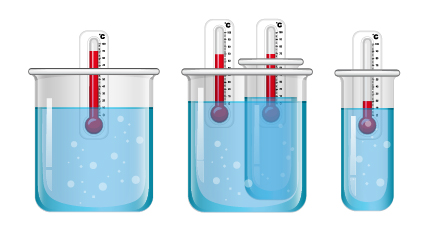
\includegraphics[width=8cm]{Images/TN8}}
\begin{itemize}
	\item Nếu ban đầu nhiệt độ của nước trong cốc thấp hơn nhiệt độ của nước ở trong bình thì sau khi đặt cốc vào trong bình quan sát thấy nhiệt độ của nước ở trong cốc tăng lên, nhiệt độ của nước ở trong bình giảm xuống, đến khi nhiệt độ của nước trong cốc và trong bình bằng nhau thì nhiệt độ của chúng được giữ ổn định.
\end{itemize}
\newghichu{Kết quả thí nghiệm cho thấy:
\begin{itemize}
	\item Các vật chỉ trao đổi nhiệt lượng cho nhau khi chúng có sự chênh lệch về nhiệt độ.
	\item Quá trình trao đổi nhiệt sẽ dừng lại khi hai vật có cùng nhiệt độ, ta nói hai vật đạt đến trạng thái cân bằng nhiệt.
\end{itemize}}
\subsubsection{Khái niệm nhiệt độ}
\newghichu{Nhiệt độ là số đo cường độ chuyển động hỗn độn của các phân tử cấu tạo nên vật.
\begin{itemize}
	\item Nhiệt độ càng cao thì các phân tử cấu tạo nên vật chuyển động nhiệt càng nhanh.
	\item Nhiệt luôn tự động truyền từ vật có nhiệt độ cao (vật nóng) sang vật có nhiệt độ thấp (vật lạnh).
	\item Nhiệt không thể tự động truyền tự vật lạnh sang vật nóng hơn.
\end{itemize}}

\begin{center}
	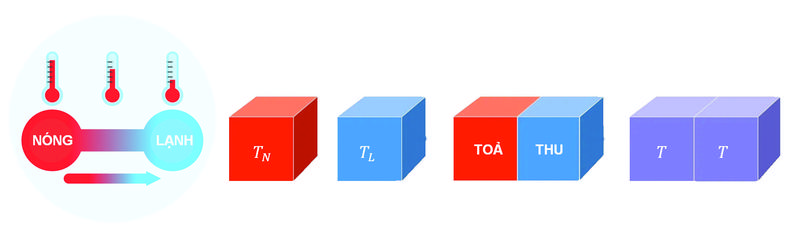
\includegraphics[width=12cm]{Images/nl2}
\end{center}
\subsection{THANG NHIỆT ĐỘ}

\setcounter{paragraph}{0}
\Binhluan{\subsubsection{Thang nhiệt độ Celsius}
\begin{itemize}
	\item Thang nhiệt độ Celsius là thang nhiệt độ có một mốc là nhiệt độ nóng chảy của nước đá tinh khiết ở áp suất 1 atm (quy ước là $0^\circ C$) và mốc còn lại là nhiệt độ sôi của nước tinh khiết ở áp suất 1 atm (quy ước là $100^\circ C$). Khoảng cách giữa hai mốc nhiệt độ này được chia thành 100 phần bằng nhau, mỗi phần ứng với $1^\circ C$.
	\item Kí hiệu: t
	\item Đơn vị: độ C ($^\circ C$). 
\end{itemize}}{Vì được chia thành 100 phần bằng nhau nên ban đầu thang nhiệt độ Celsius còn được gọi là \textit{thang nhiệt độ bách phân}}
%\vspace*{-1 cm}
\subsubsection{Thang nhiệt độ Kelvin}
\begin{itemize}
	\item Trong thang nhiệt độ Kelvin, mọi nhiệt độ trong đó đều có giá trị dương. Hai nhiệt độ được dùng làm mốc là:
	\immini{\begin{itemize}
		\item Nhiệt độ thấp nhất mà các vật có thể có. Không có vật ở bất kì trạng thái nào có thể có nhiệt độ thấp hơn nhiệt độ này. Nhiệt độ này được gọi là \textit{"Độ không tuyệt đối"}. 
		\item Nhiệt độ mà nước đá, nước và hơi nước có thể cùng tồn tại, được định nghĩa là  273,16 K (tương đương với $0,01^\circ C$). Hay còn được gọi là nhiệt độ điểm ba của nước.
	\end{itemize} }{
\begin{tikzpicture}
\tkzDefPoints{0/0/a, 6/0/b, 6/4/c, 0/4/d}
\fill[cyan!80!white] (0,0) .. controls (0.79,0.2) and (1.18,0.41) .. (1.5,1)--(1,4)--(d);
\draw (0,0) .. controls (0.79,0.2) and (1.18,0.41) .. (1.5,1);
\fill[cyan!40!white] (1.5,1) .. controls (3.42,1.14) and (4.16,1.93) .. (5.5,4)--(1,4)--cycle;
\draw (1.5,1) .. controls (3.42,1.14) and (4.16,1.93) .. (5.5,4);
\draw (1,4) --(1.5,1);
\draw[dashed] (0,1)node[above,rotate=90]{\scriptsize 611,73} --(1.5,1);
\draw[dashed] (1.5,0)node[below]{\scriptsize 0,01} --(1.5,1);
\node[below] at (5,0){\scriptsize Nhiệt độ ($^\circ C$)};
\node[left,rotate=90] at (-0.25,4){\scriptsize Áp suất ($Pa$)};
\node at (3,3){\scriptsize Nước};
\node[white]  at (0.6,2.5){\scriptsize Nước đá};
\node at (4.5,1){\scriptsize Hơi nước};
\tkzDrawPolygon[](a,b,c,d)
\node at (3,-1){Đồ thị biểu diễn điểm ba của nước};
\end{tikzpicture}
}
\item Kí hiệu: T
\item Đơn vị: Kelvin (K).
\end{itemize}
\begin{note}
	\begin{itemize}
	\item 0 K là nhiệt độ mà các phân tử có \textit{động năng chuyển động nhiệt bằng không} và \textit{thế năng tương tác giữa chúng là tối thiểu}. Nghĩa là hệ ở 0 K sẽ có nội năng tối thiểu. 
	\item 0 K tương đương với $-273,15^\circ C$.
	\item Mỗi độ chia (1 K)  trong thang nhiệt độ Kelvin có độ lớn bằng $\dfrac{1}{273,16}$ khoảng cách giữa hai nhiệt độ mốc của thang nhiệt độ này.
\end{itemize}
\end{note}
\subsubsection{Thang nhiệt độ Fahrenheit}
Thang nhiệt độ Fahrenheit được nhà vật lí người Đức là Daniel Gabriel Fahrenheit (Đa-ni-en Ga-ri-eo Fa-ren-hai) đề xuất vào năm 1724. \immini{Ông chọn hai mốc nhiệt độ tương ứng với nhiệt độ của nước đá đang tan ở áp suất 1 atm là $32^\circ F$ và nhiệt độ sôi của nước tinh khiết ở áp suất 1 atm là $212^\circ F$. Trong khoảng giữa hai mốc nhiệt độ này, chia thành 180 khoảng bằng nhau, mỗi khoảng ứng với $1^{\circ} F$. Thang đo này được sử dụng phổ biến ở các nước phương Tây. Nếu gọi $t$ là nhiệt độ của vật trong thang nhiệt độ Celcius và $T$ là nhiệt độ của vật trong thang nhiệt độ Fahrenheit thì:
$$
T\left({ }^\circ F\right)=1,8 t\left(^\circ C\right)+32
$$
}{
\includegraphics[width=4cm]{images/112317}}

\Binhluan{\subsection{CHUYỂN ĐỔI GIỮA CÁC THANG ĐO}
	
\begin{itemize}
	\item T (K): Giá trị nhiệt độ theo thang Kelvin
	\item $t\ (^\circ C)$: Giá trị nhiệt độ theo thang Celcius
	\item $t\ (^\circ F)$: Giá trị nhiệt độ theo thang Fahrenheit 
\end{itemize}
\begin{align*}
\boder{T\ (K)=t\ (^\circ C)+273,15\approx t\ (^\circ C)+273}
\end{align*}
\begin{align*}
\boder{t\ (^\circ F)=32+1,8.t\ (^\circ C)}
\end{align*}}{Sự chênh lệch nhiệt độ của thang nhiệt Celsius ($^\circ C$)  và thang nhiệt Kelvin (K)  là như nhau
	$$(t_2-t_1)\ ^\circ C = (T_2-T_1)\ K$$
}
\begin{center}
	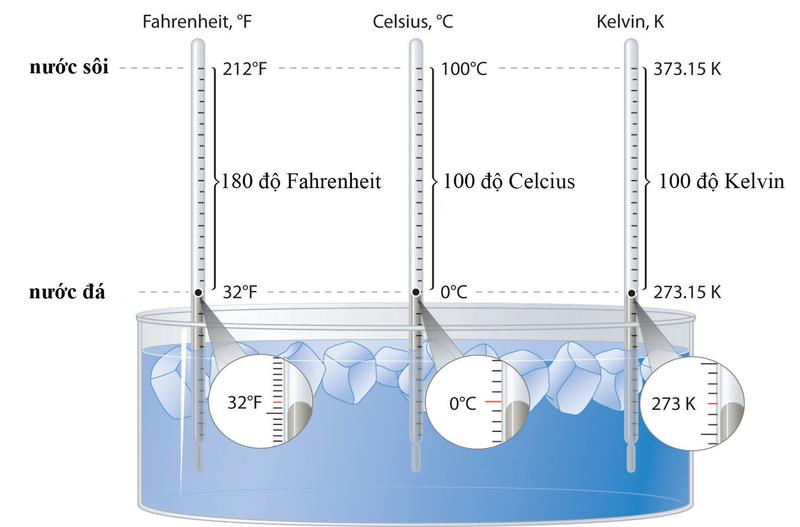
\includegraphics[width=12cm]{Images/thangdonhietdo}
\end{center}
\subsection{NHIỆT KẾ}

\setcounter{paragraph}{0}
\subsubsection{Khái niệm}
\textbf{Nhiệt} kế là thiết bị dùng để đo nhiệt độ. Nhiệt kế được chế tạo dựa trên một số tính chất vật lí phụ thuộc vào nhiệt độ của các chất, các vật liệu, các linh kiện điện và điện tử,...
\subsubsection{Một số loại nhiệt kế thường gặp}
\immini{\begin{itemize}
\item \textbf{Nhiệt kế chất lỏng:} Hoạt động dựa vào sự giãn nở nhiệt của một số chất lỏng (thuỷ ngân, rượu, dầu,…). Thông qua việc xác định độ cao của cột chất lỏng ở các nhiệt độ khác nhau, ta có thể xác định được nhiệt độ cần đo.
\end{itemize} }{	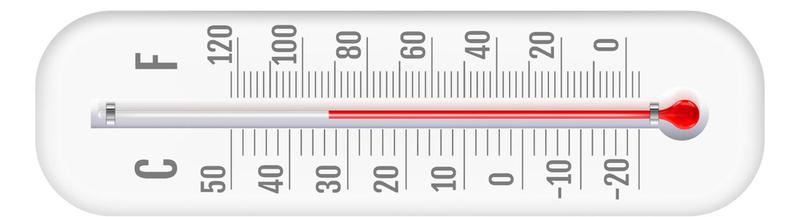
\includegraphics[width=3cm]{Images/nhietkelong}}
\immini{\begin{itemize}
	\item \textbf{Nhiệt kế khí:} Hoạt động dựa vào sự nở vì nhiệt của một lượng khí xác định ở áp suất không đổi. 
\end{itemize} }{	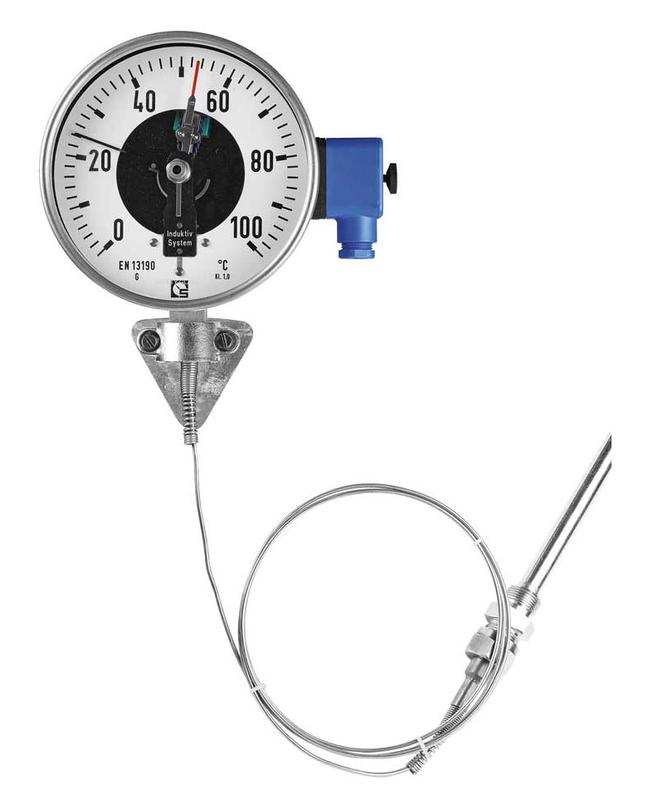
\includegraphics[width=3cm]{Images/nhietkekhi}}
\immini{\begin{itemize}
	\item \textbf{Nhiệt kế kim loại:} Hoạt động dựa vào sự nở dài của một thanh kim loại mỏng hoặc xoắn ốc. 
\end{itemize} }{	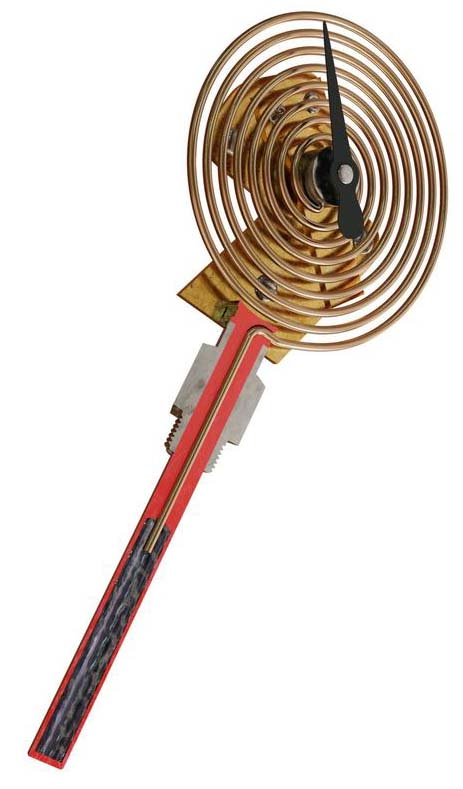
\includegraphics[width=3cm]{Images/nhietkekimloai}}
\immini{\begin{itemize}
\item \textbf{Nhiệt kế điện trở:} Hoạt động dựa vào sự phụ thuộc của điện trở vào nhiệt độ. 
\end{itemize} }{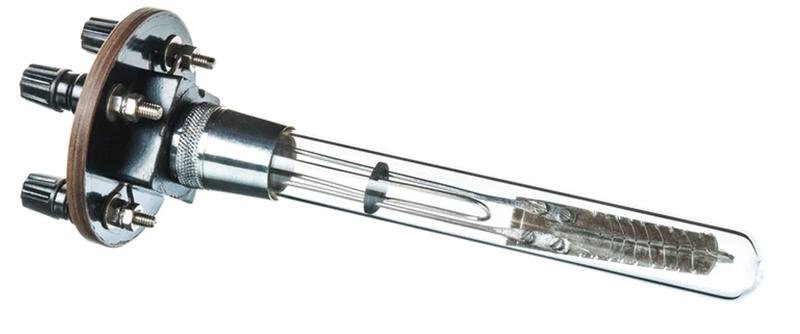
\includegraphics[width=3cm]{Images/nhietkedientro1}}
\immini{\begin{itemize}
	\item \textbf{Nhiệt kế nhiệt điện:} Hoạt động dựa vào suất điện động nhiệt điện giữa hai mối hàn của hai kim loại khác bản chất. 
\end{itemize} }{	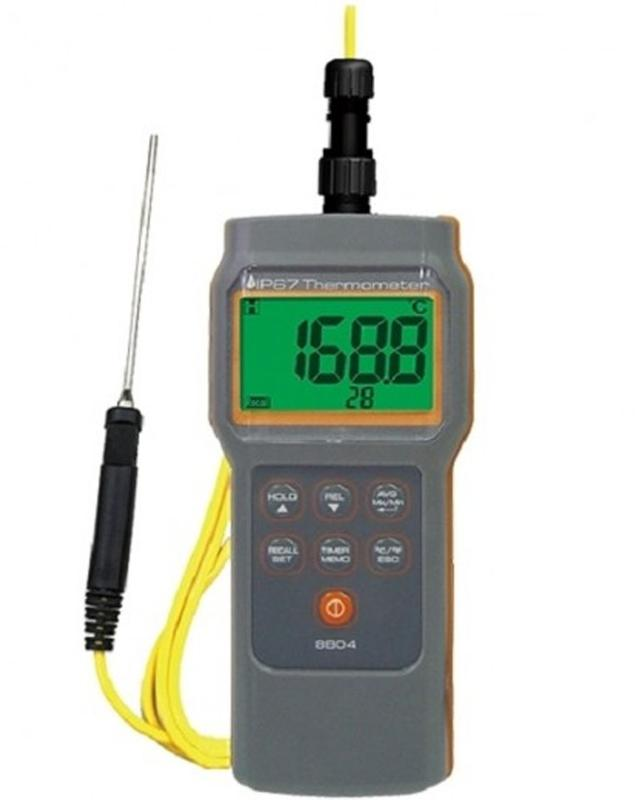
\includegraphics[width=3cm]{Images/nhietkenhietdien}}
\immini{\begin{itemize}
	\item \textbf{Nhiệt kế hồng ngoại:} Hoạt động dựa vào sự phụ thuộc vào nhiệt độ của bước sóng bức xạ hồng ngoại do vật phát ra.	
\end{itemize} }{	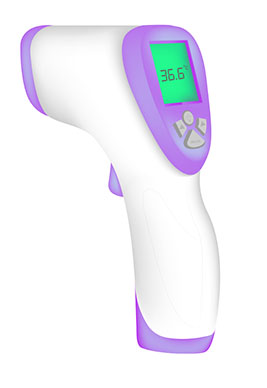
\includegraphics[width=3cm]{Images/nhietkedientu}}











